\documentclass{beamer}
\input{config/rc-slides-config.tex}
\usepackage[english]{babel}
\usepackage{amsfonts}
\usepackage{amsmath}
\usepackage{amssymb}
\usepackage{bm}
%\usepackage{subfig}
\usepackage{graphicx}
\usepackage{array}
\usepackage{natbib}
%\usepackage{caption}
% \usepackage{mathtools}
% \usepackage{algorithm}
% \usepackage{algorithmic}
%\usepackage{tabularx}
%\usepackage{xltabular}  
\usepackage{booktabs} 
\usepackage{xcolor}
\usepackage{makecell}
\usepackage{lipsum}
\usepackage{multirow}
% \usepackage{tikz} 
%\usepackage{minted}
% \usepackage{setspace}
\usepackage{hyperref}

\title[Secondary patterns]{POM: Evaluating model's capability to reproduce multiple patterns}
\institute[UV]{\textbf{Instituto de Investigaciones en Inteligencia Artificial} \\ Universidad Veracruzana \\ \vspace{0.25cm} \emph{Campus Sur, Calle Paseo Lote II, Sección Segunda No 112, \\ Nuevo Xalapa, Xalapa, Ver., México 91097}  \\ 
	\vspace{0.25cm}   
}
\author[Ulises J. G.]{Ulises Jiménez Guerrero}
\date[MIA 2026]{\today}

\logo{
	
\includegraphics[width=0.8cm]{figs/logo_UV.png} 
}

%\usetheme{CambridgeUS}

\begin{document}
	
\begin{frame}
	\maketitle
\end{frame}
		
\section{Objectives}

\begin{frame}{Objectives}
	\begin{itemize}
		\item An ABM opinion dynamics model was developed to reproduce the opinion change during the Mexican 2024 presidential election. It was found to be capable of reproducing the main pattern considered: empirical preference share registered in a selected opinion poll.
		
		\item For the current experiments, we follow Pattern Oriented Modeling (POM) \cite{railsbackAgentbasedIndividualbasedModeling2019} and evaluate the model's capability to reproduce multiple patterns observed in an election, such as vote share by gender and age group.
	\end{itemize}
\end{frame}

\begin{frame}{Structural realism}
	\begin{itemize}
		\item An ABM should be as simple as possible while still capturing and reproducing the key characteristics and behaviors of the real system, based on the objectives of the simulation.
		
		\item This is called \emph{structural realism}: including only the essential components of a real system that are needed to produce the main properties and behaviors. 
	\end{itemize}
\end{frame}

\begin{frame}{Pattern Oriented Modeling (POM)}
	\begin{itemize}
		\item A model can be capable of reproducing the main pattern observed in a phenomena while not having structural realism.
		
		\item POM helps to identify the main components necessary in the model, by using \emph{multiple} observed patterns in the real system. A model capable of reproducing multiple patterns is more likely to have achieved structural realism.
	\end{itemize}
\end{frame}

\section{Materials and methods}
\begin{frame}{Chosen opinion polls}
	\begin{itemize}
		\item The proposed model is based on the study carried over by the group GEA-ISA for the election analyzed \cite{gea2024estudios}. It reports the voting intention of 1070 mexican citizens interviewed at a nationwide scale, registering multiple demographic variables. 
		
		\item The data was adjusted to consider only the two main candidates. The election results were also considered, and the resulting preference share is as shown in the following table.
	\end{itemize}
	\centering
	\begin{table}
		\resizebox{1 \textwidth}{!}{
			\begin{tabular}{|c|c|c|c|}
				\hline
				\textbf{Date} & 
				\textbf{Time (days)} & 
				\textbf{Preference for A (\%)} & 
				\textbf{Preference for B (\%)} 
				\\
				\hline
				2023/09/16 &
				0  &
				61  & 
				39
				\\ 
				\hline
				2023/11/25 &
				70  &
				64  &
				36
				\\
				\hline 
				2024/03/01 &
				167  &
				61 &
				39 \\
				\hline 
				\textbf{(Election day) 2024/06/02} &
				260  &
				68 &
				32 \\
				\hline
			\end{tabular}
		}	
	\end{table}
\end{frame}

\begin{frame}{Basic model}
	\begin{itemize}
		\item A basic model of opinion dynamics was developed considering the poll's characteristics and the restrictions of a political election. The model considers three different types of influence, based on a classification given by \cite{flacheModelsSocialInfluence2017b, smaldinoModelingSocialBehavior2023}.
		
		\item The model consist of 1070 individual, with every time step representing a day. As such, a run consist of 260 time steps or ticks, considering the days since the first poll until the election day. The initial preference share is taken from the first available poll.
		
		\item The model was capable of reproducing the main pattern of preference share at the three dates with empirical data.
	\end{itemize}	
\end{frame}

\begin{frame}{Limitations of the basic model}
	\begin{itemize}
		\item The developed basic model doesn't consider any characteristic for the agents besides their initial preference. As such, the only pattern capable to be validated is the preference share.
		
		\item To validate multiple patterns, the model needs to be modified so the agents have multiple characteristics beyond their opinion. This is done considering age and gender.
	\end{itemize}
	
	\begin{figure}[h!]
		\centering
		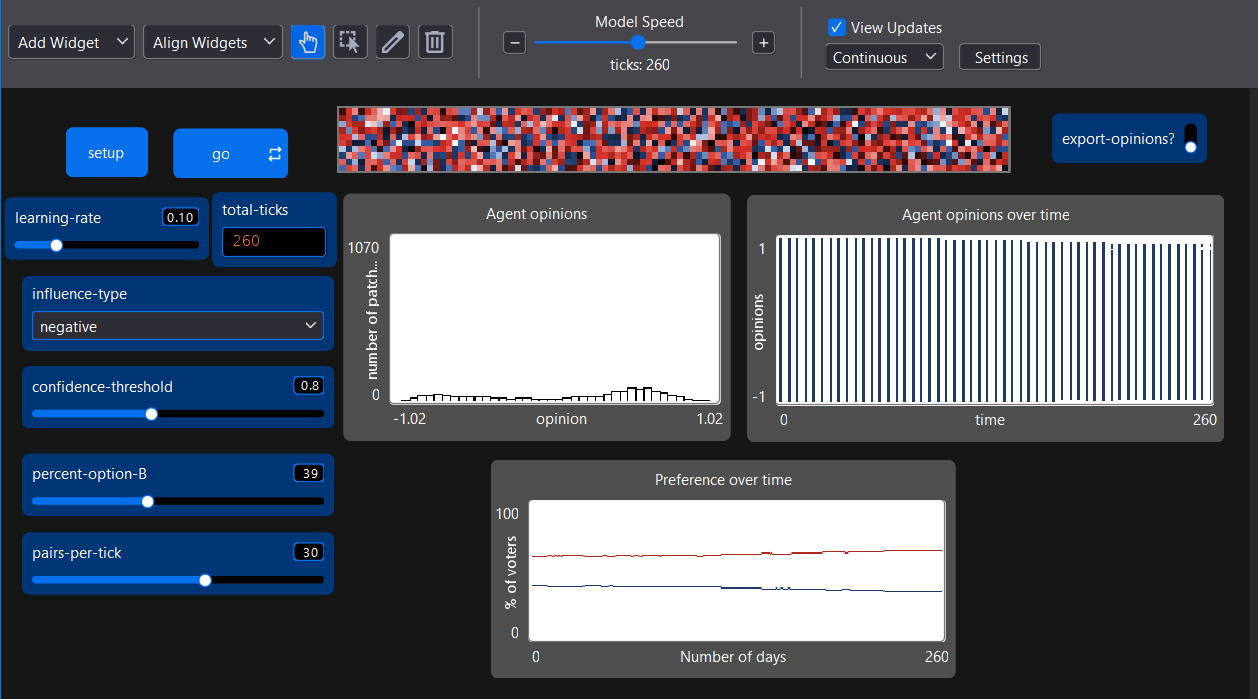
\includegraphics[width=0.6\linewidth]{figs/basic_model_2}
		\label{fig:basicmodel2}
	\end{figure}
	
\end{frame}

\begin{frame}{Obtaining preference share by gender}
	\begin{itemize}
		\item Survey data is weighted to represent the proportions reported in the national electoral list, and this was taken into account while reducing the data to the two main options.
		
		\item The electoral registry shows an electorate composed of $48\%$ men and $52 \%$ women. 
		
		\item The preference share by gender was calculated for each one of the available polls, first dividing the population by gender and then calculating each subgroup preferences.
	\end{itemize}
\end{frame}
%
%\begin{frame}{Preference share by gender in first poll}
%	\begin{figure}[h!]
%		\centering
%		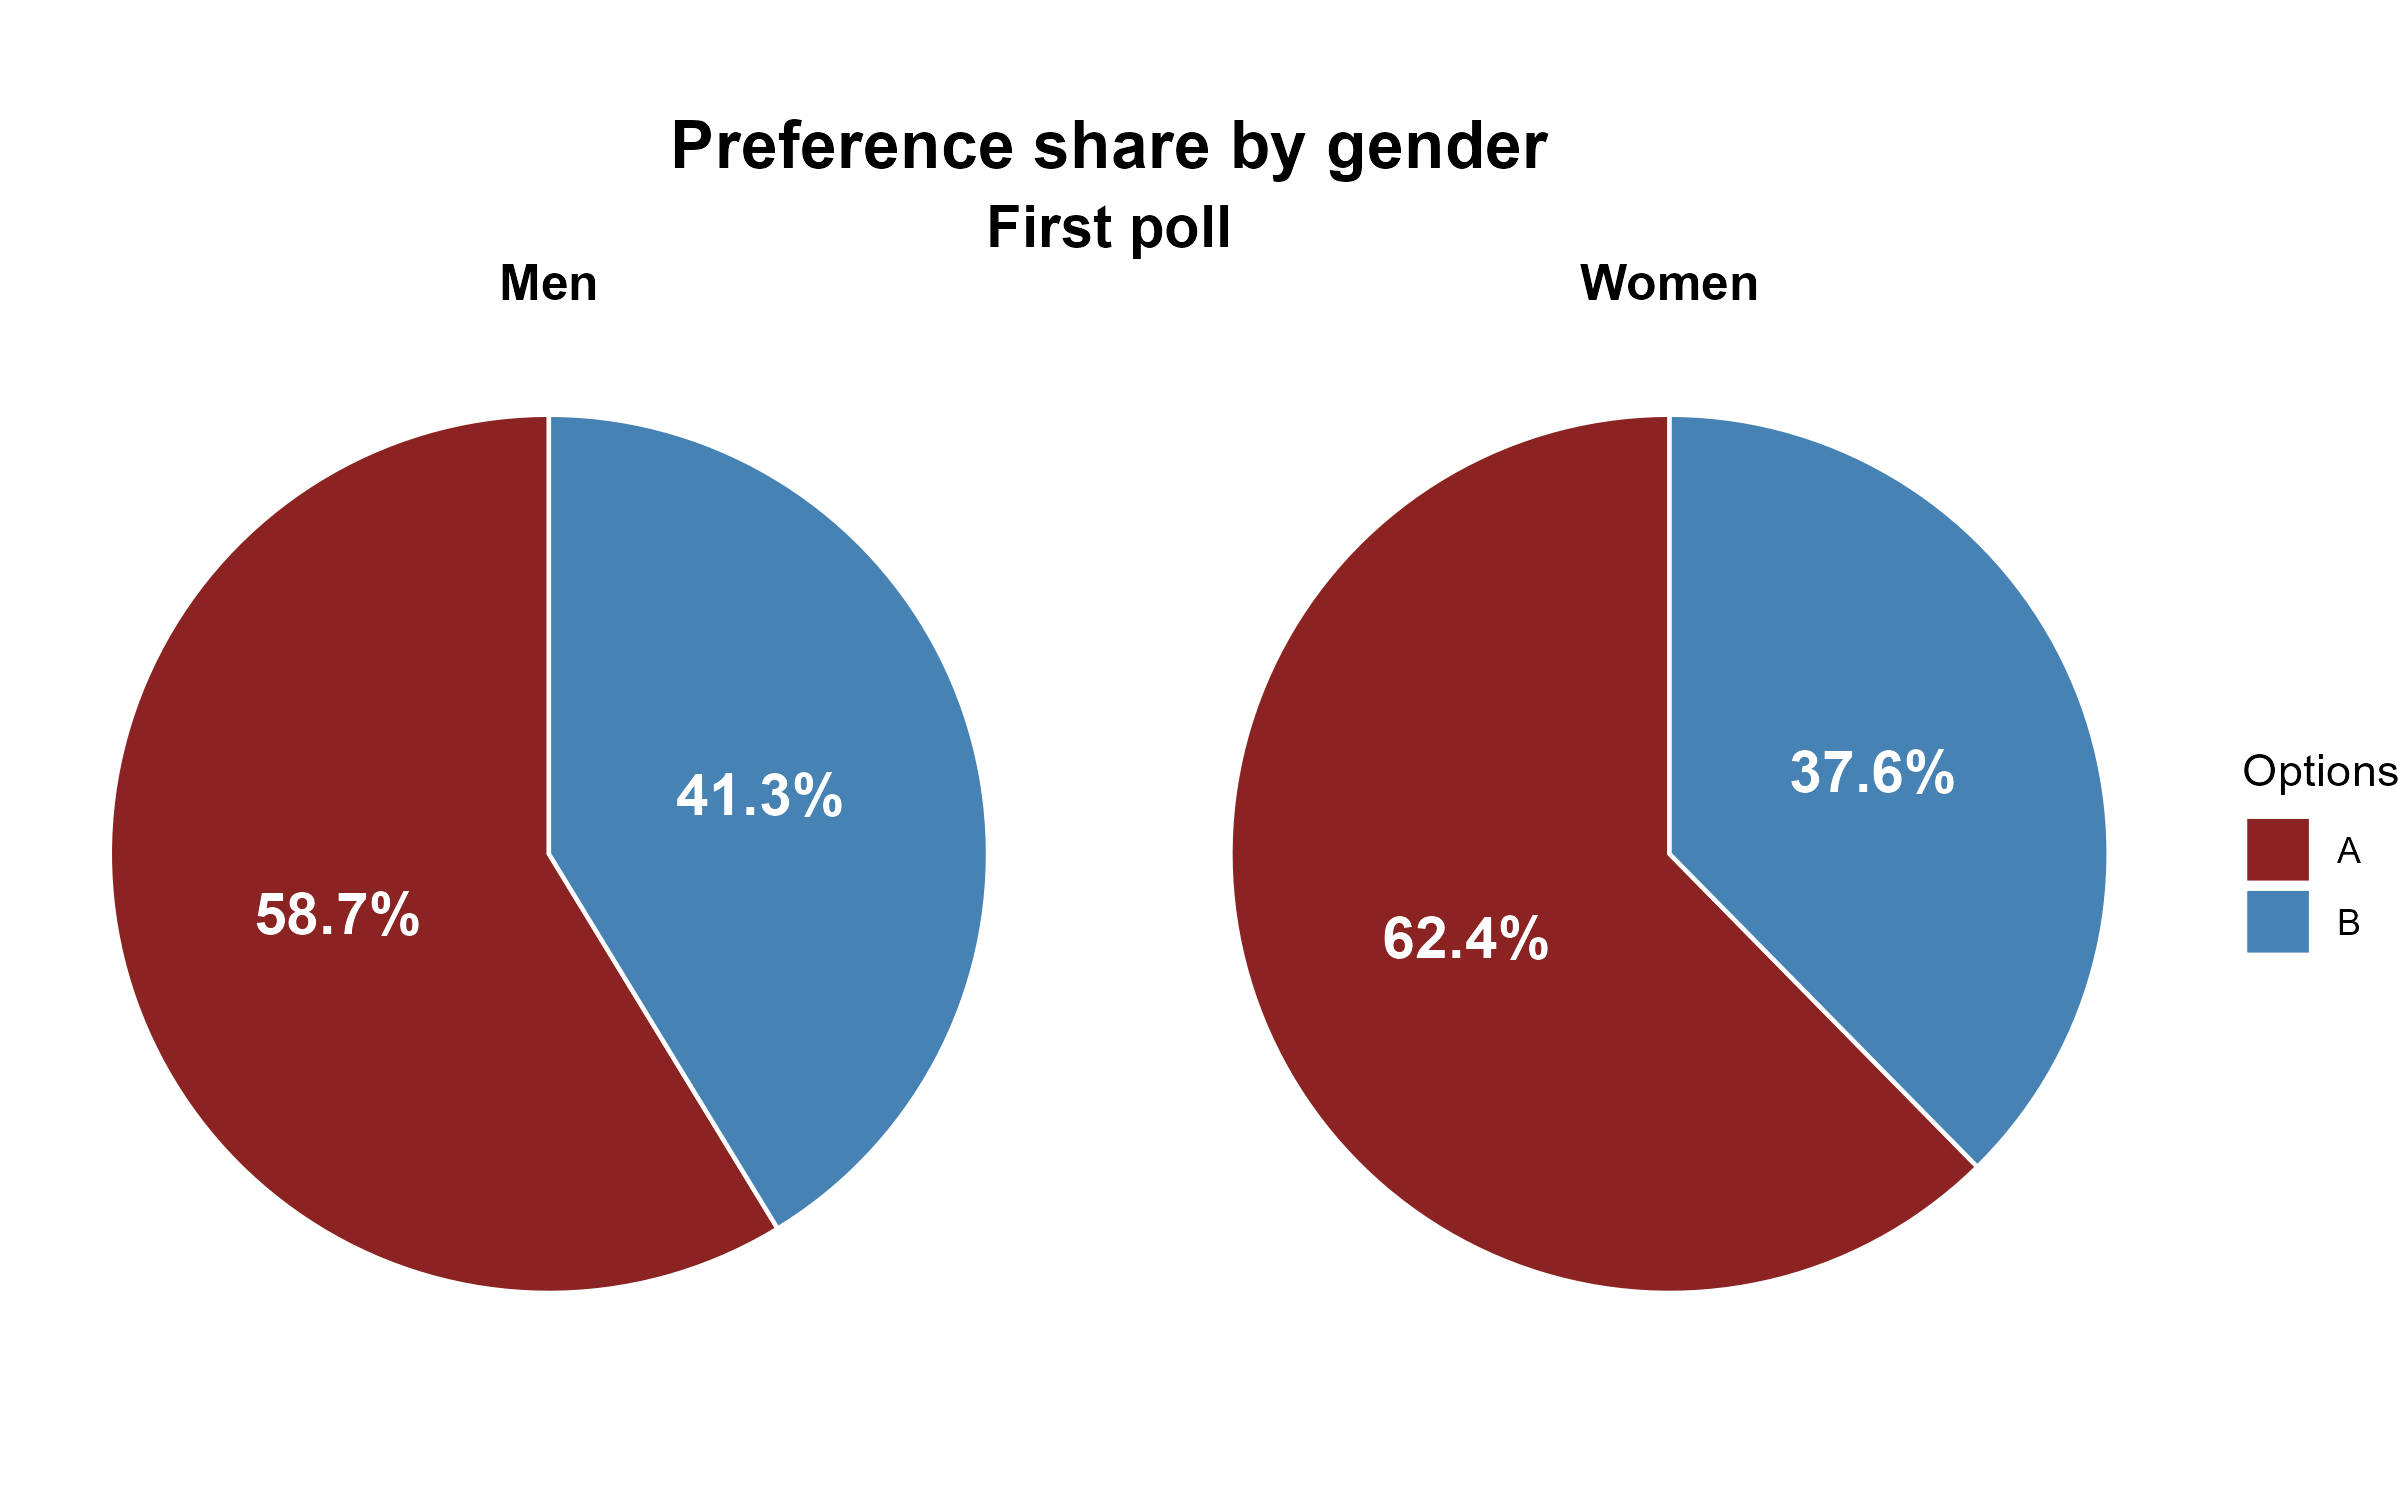
\includegraphics[width=1\linewidth]{figs/first_poll_preference_share_gender}
%	\end{figure}
%\end{frame}
%
%\begin{frame}{Preference share by gender in second poll}
%	\begin{figure}[h!]
%		\centering
%		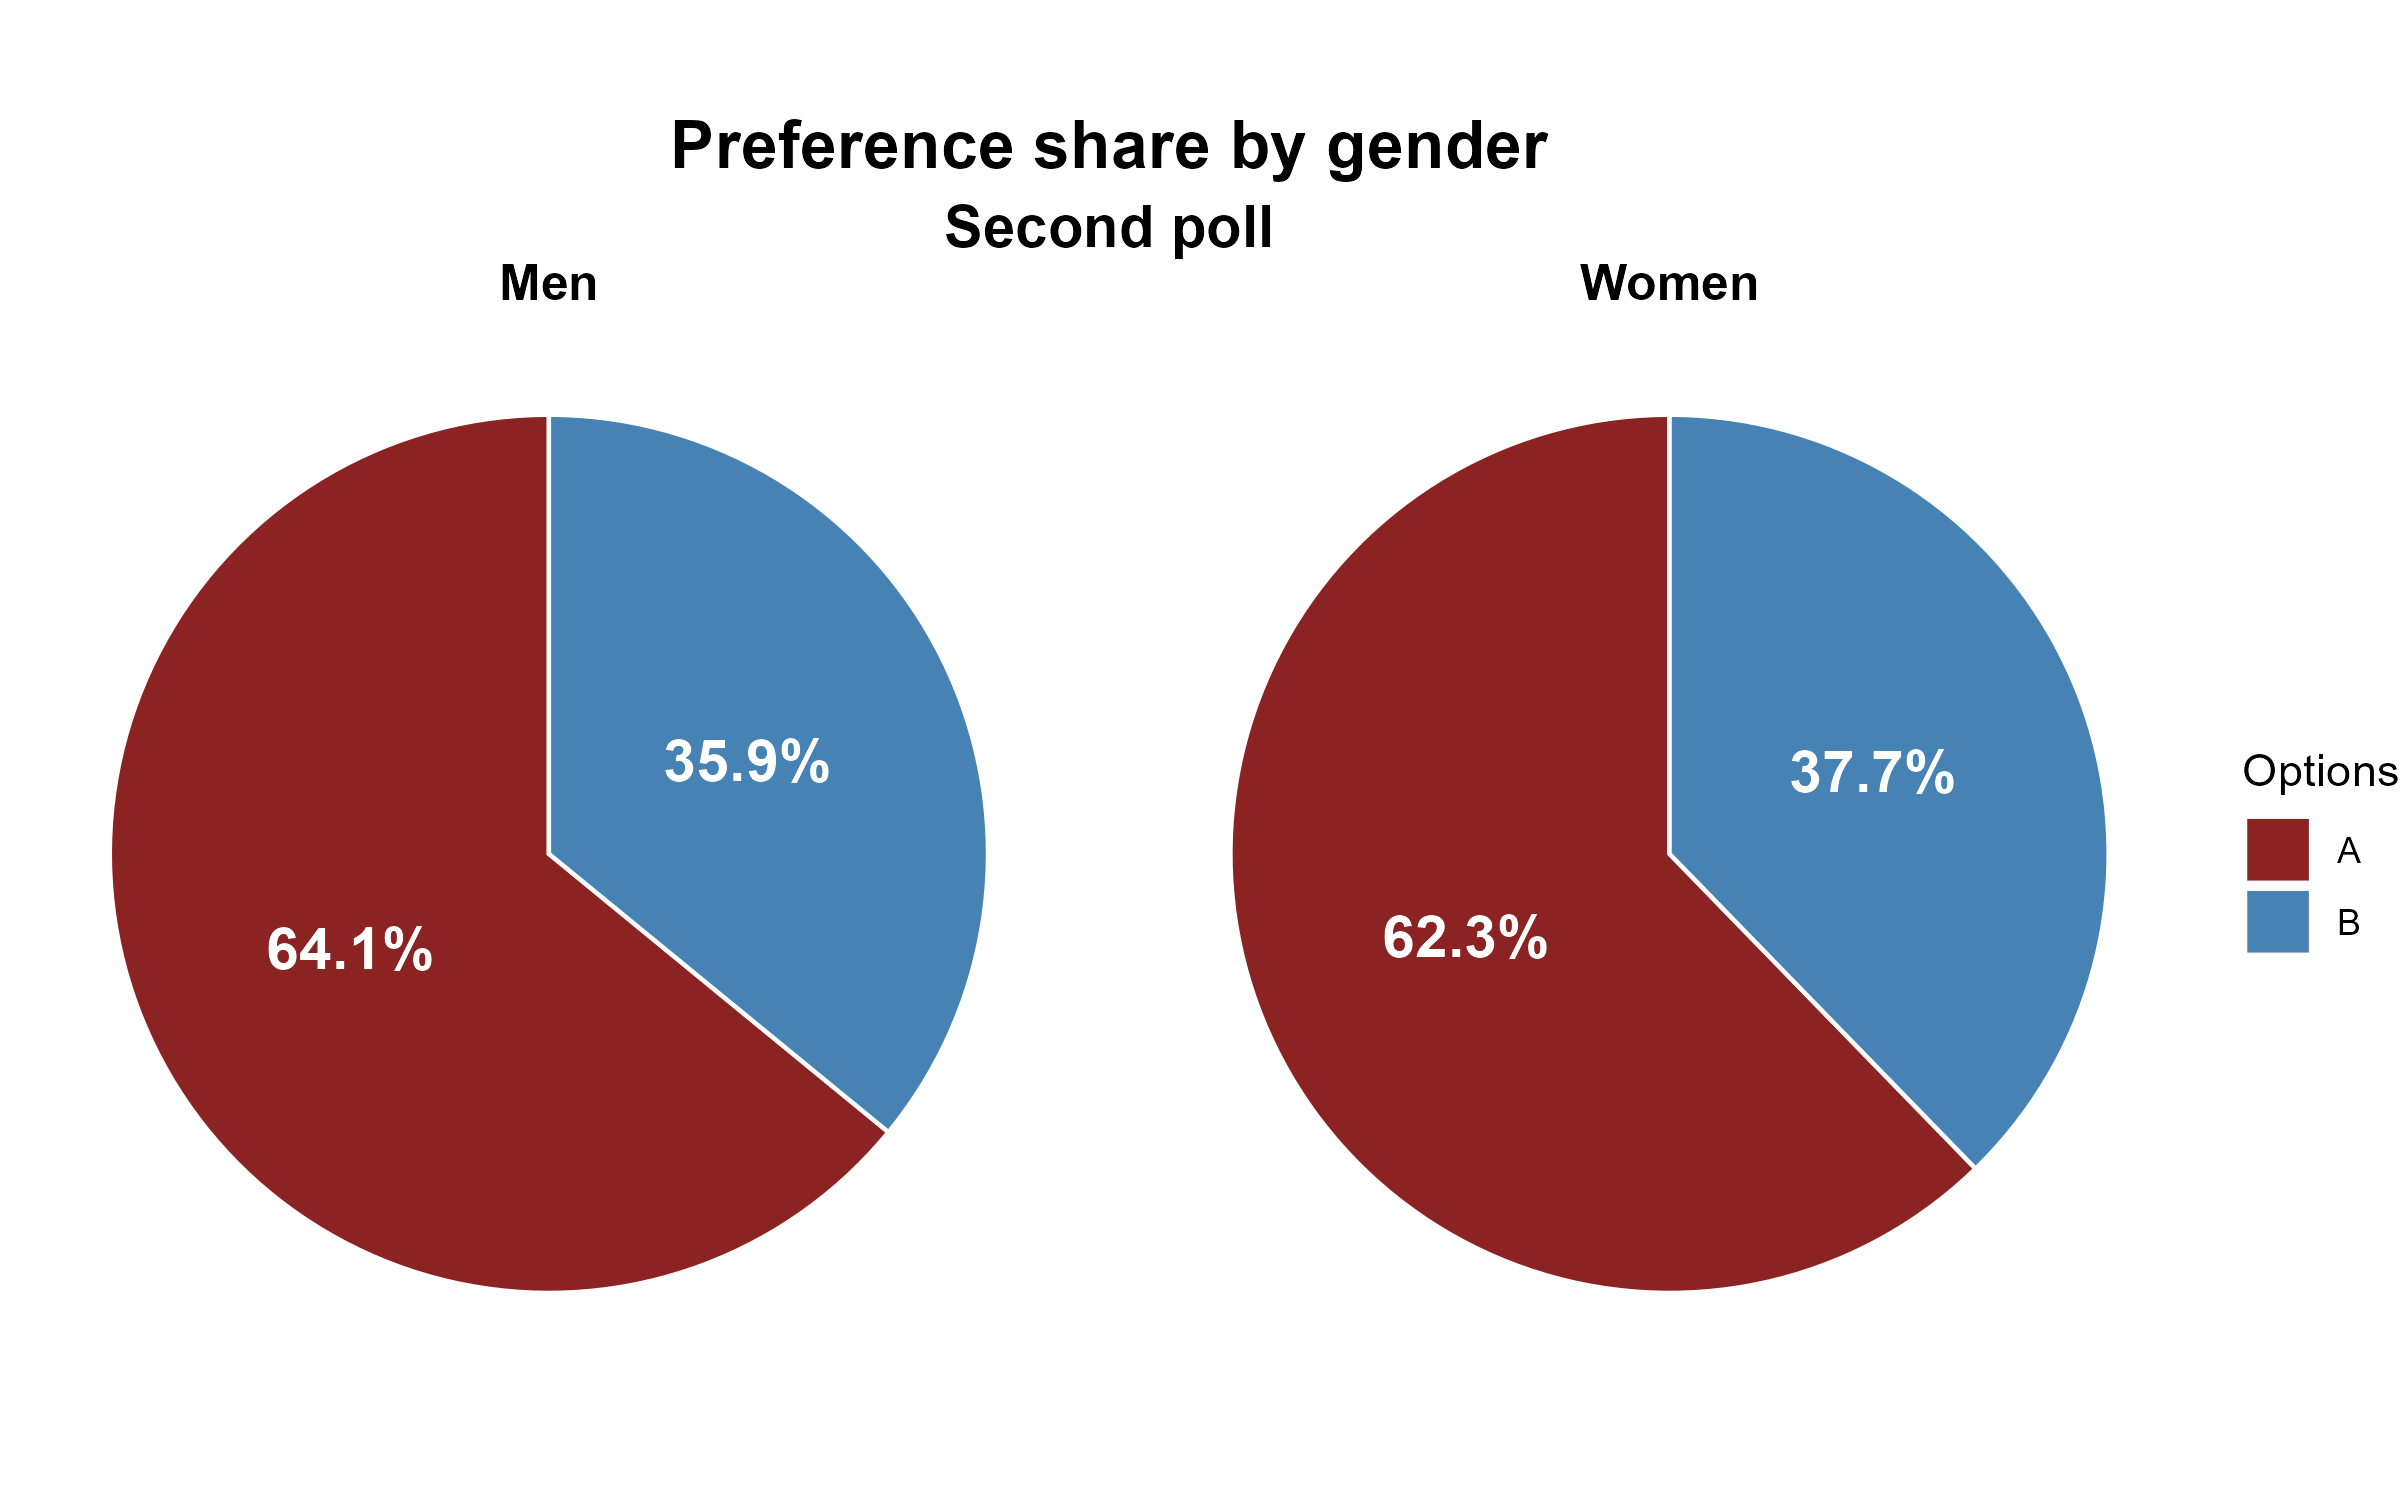
\includegraphics[width=1\linewidth]{figs/second_poll_preference_share_gender}
%	\end{figure}
%\end{frame}
%
%\begin{frame}{Preference share by gender in third poll}
%	\begin{figure}[h!]
%		\centering
%		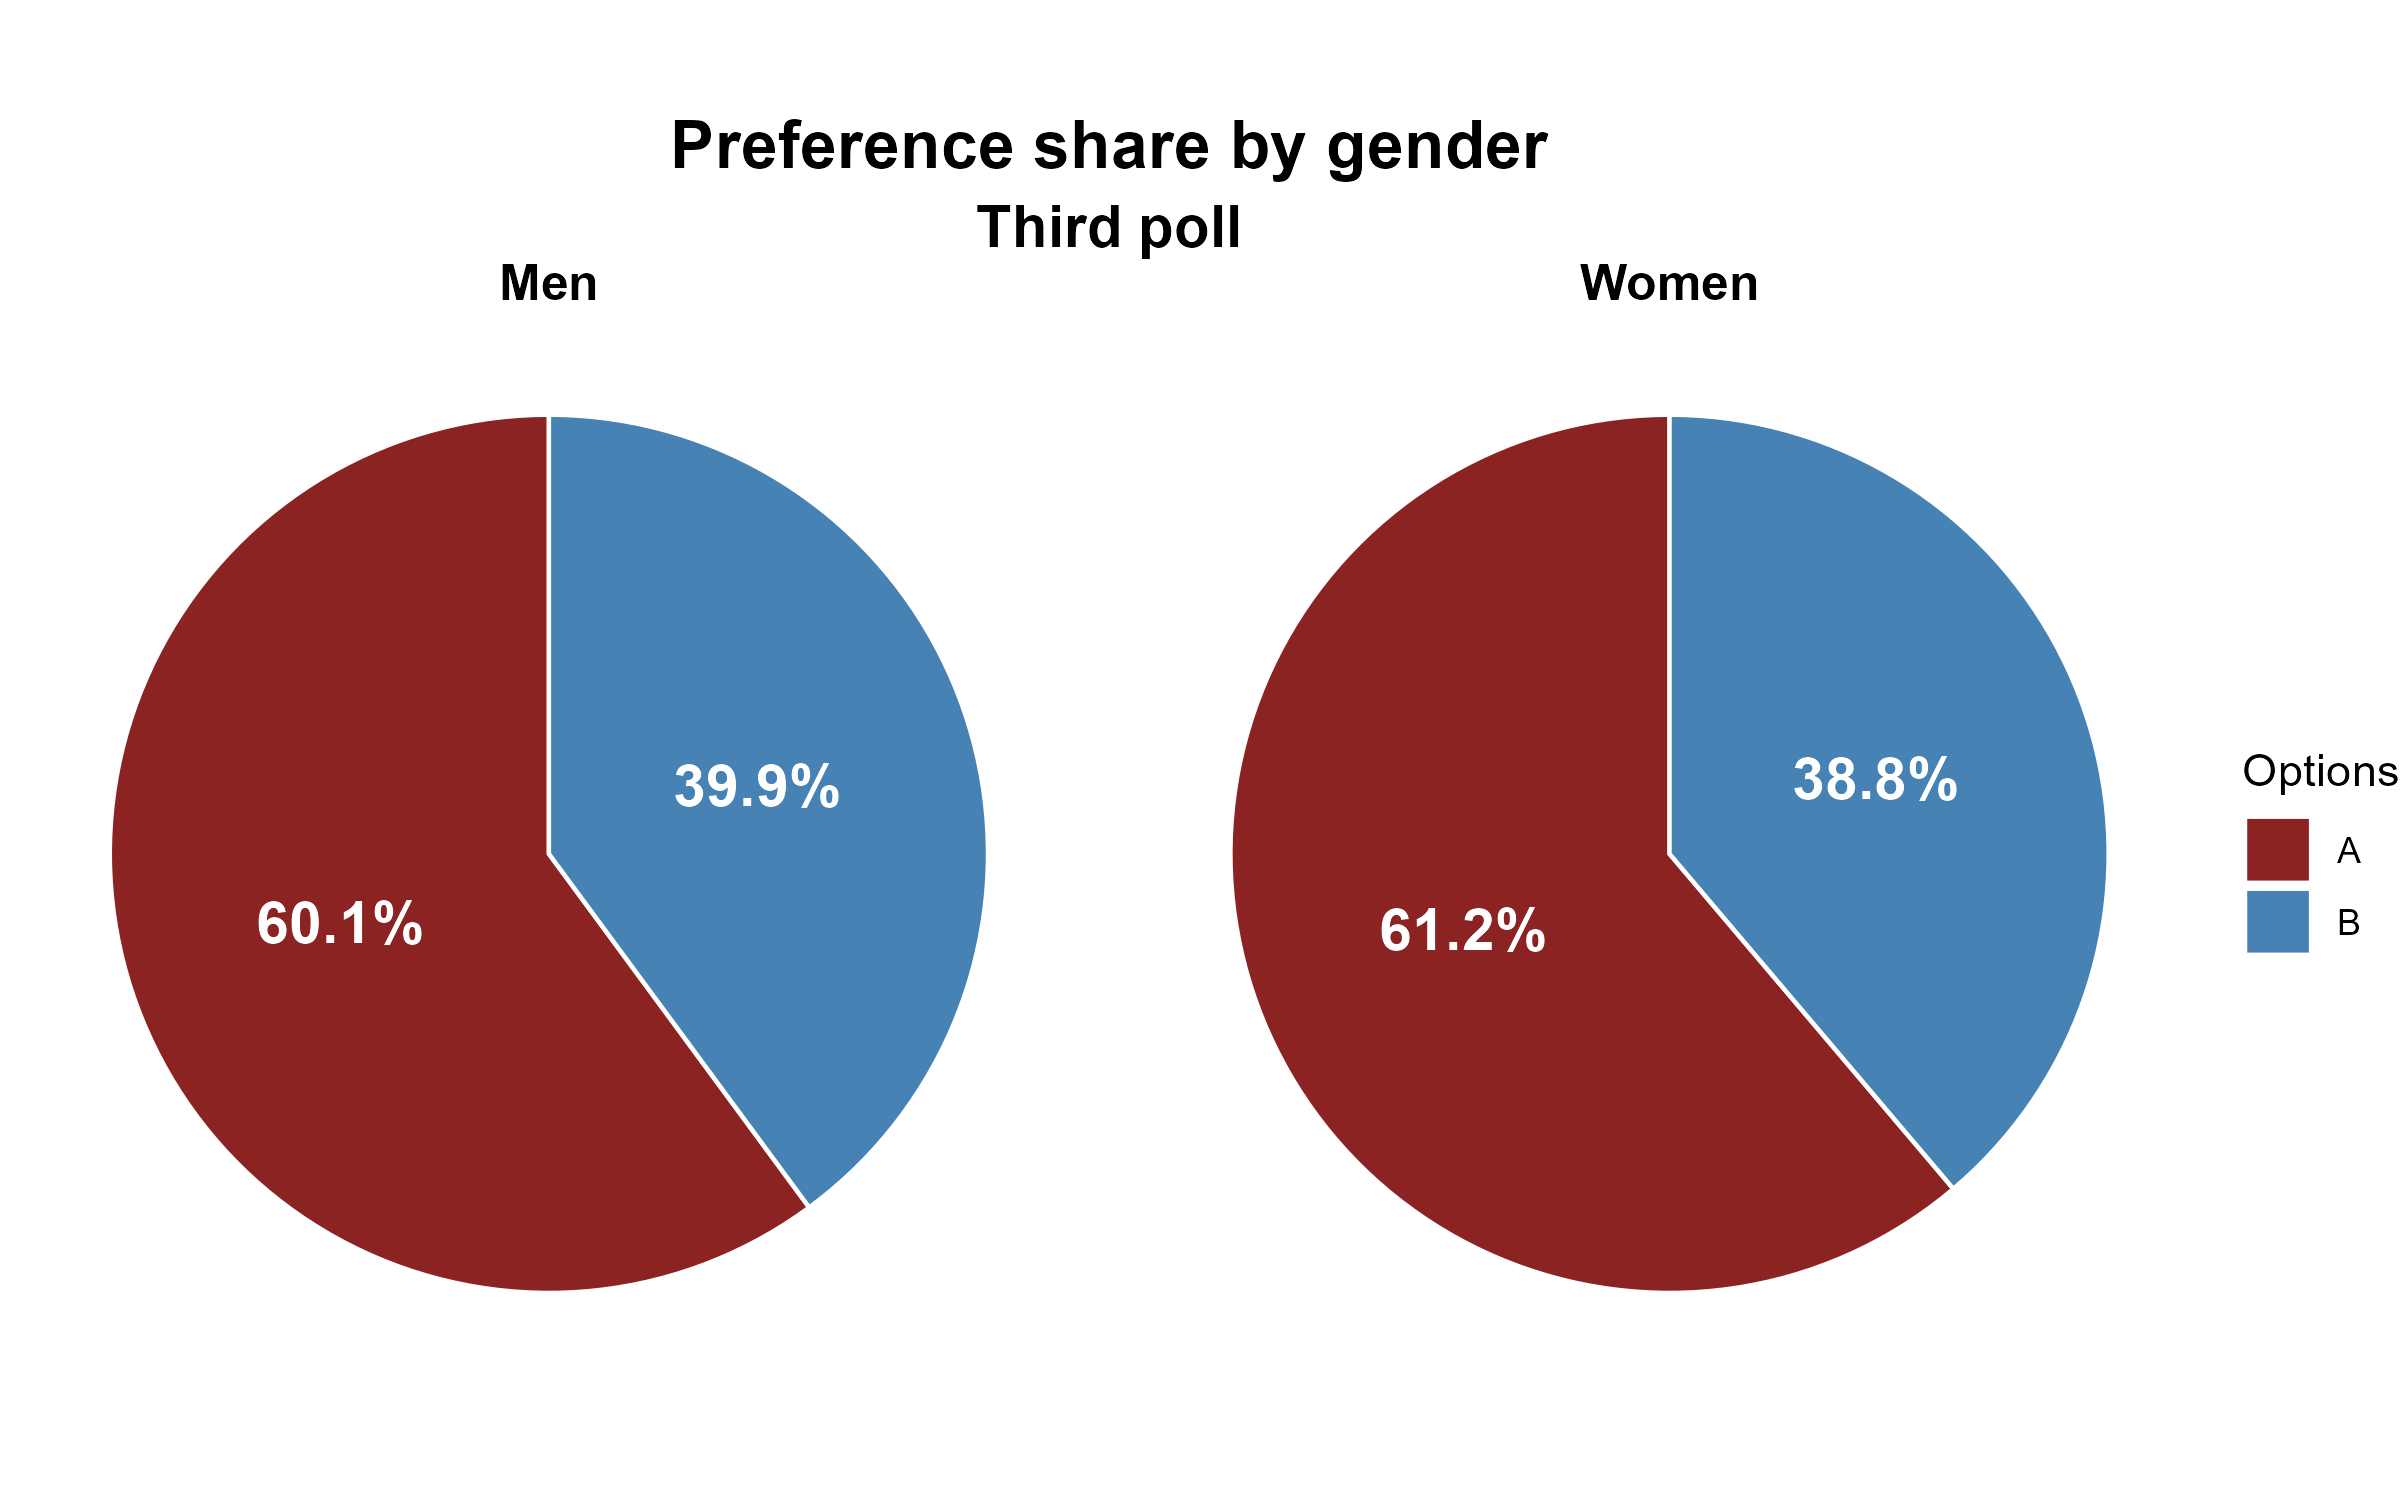
\includegraphics[width=1\linewidth]{figs/third_poll_preference_share_gender}
%	\end{figure}
%\end{frame}


\begin{frame}{Evolution of preference share by gender}
	The evolution of the preference share for both genders is shown in the following table. We see almost no change for women, while men show an overall increase of support for B, which we seek to see replicated in the model.
	\begin{table}[h]
		\centering
	\resizebox{0.8 \textwidth}{!}{
		\begin{tabular}{llccc}
			\toprule
			\textbf{Gender} & \textbf{Option} & \textbf{Survey 1 (\%)} & \textbf{Survey 2 (\%)} & \textbf{Survey 3 (\%)} \\ 
			\midrule
			\multirow{2}{*}{Men}   & Option A & $58.7$ & $64.1$ & $60.1$ \\
			& Option B & $41.3$ & $35.9$ & $39.9$ \\ 
			\cmidrule{1-5}
			\multirow{2}{*}{Women} & Option A & $62.4$ & $62.3$ & $61.2$ \\
			& Option B & $37.6$ & $37.7$ & $38.8$ \\ 
			\bottomrule
		\end{tabular}
	}
	\end{table}
\end{frame}

\begin{frame}{Evolution of preference share for men}
	\begin{figure}[h!]
		\centering
		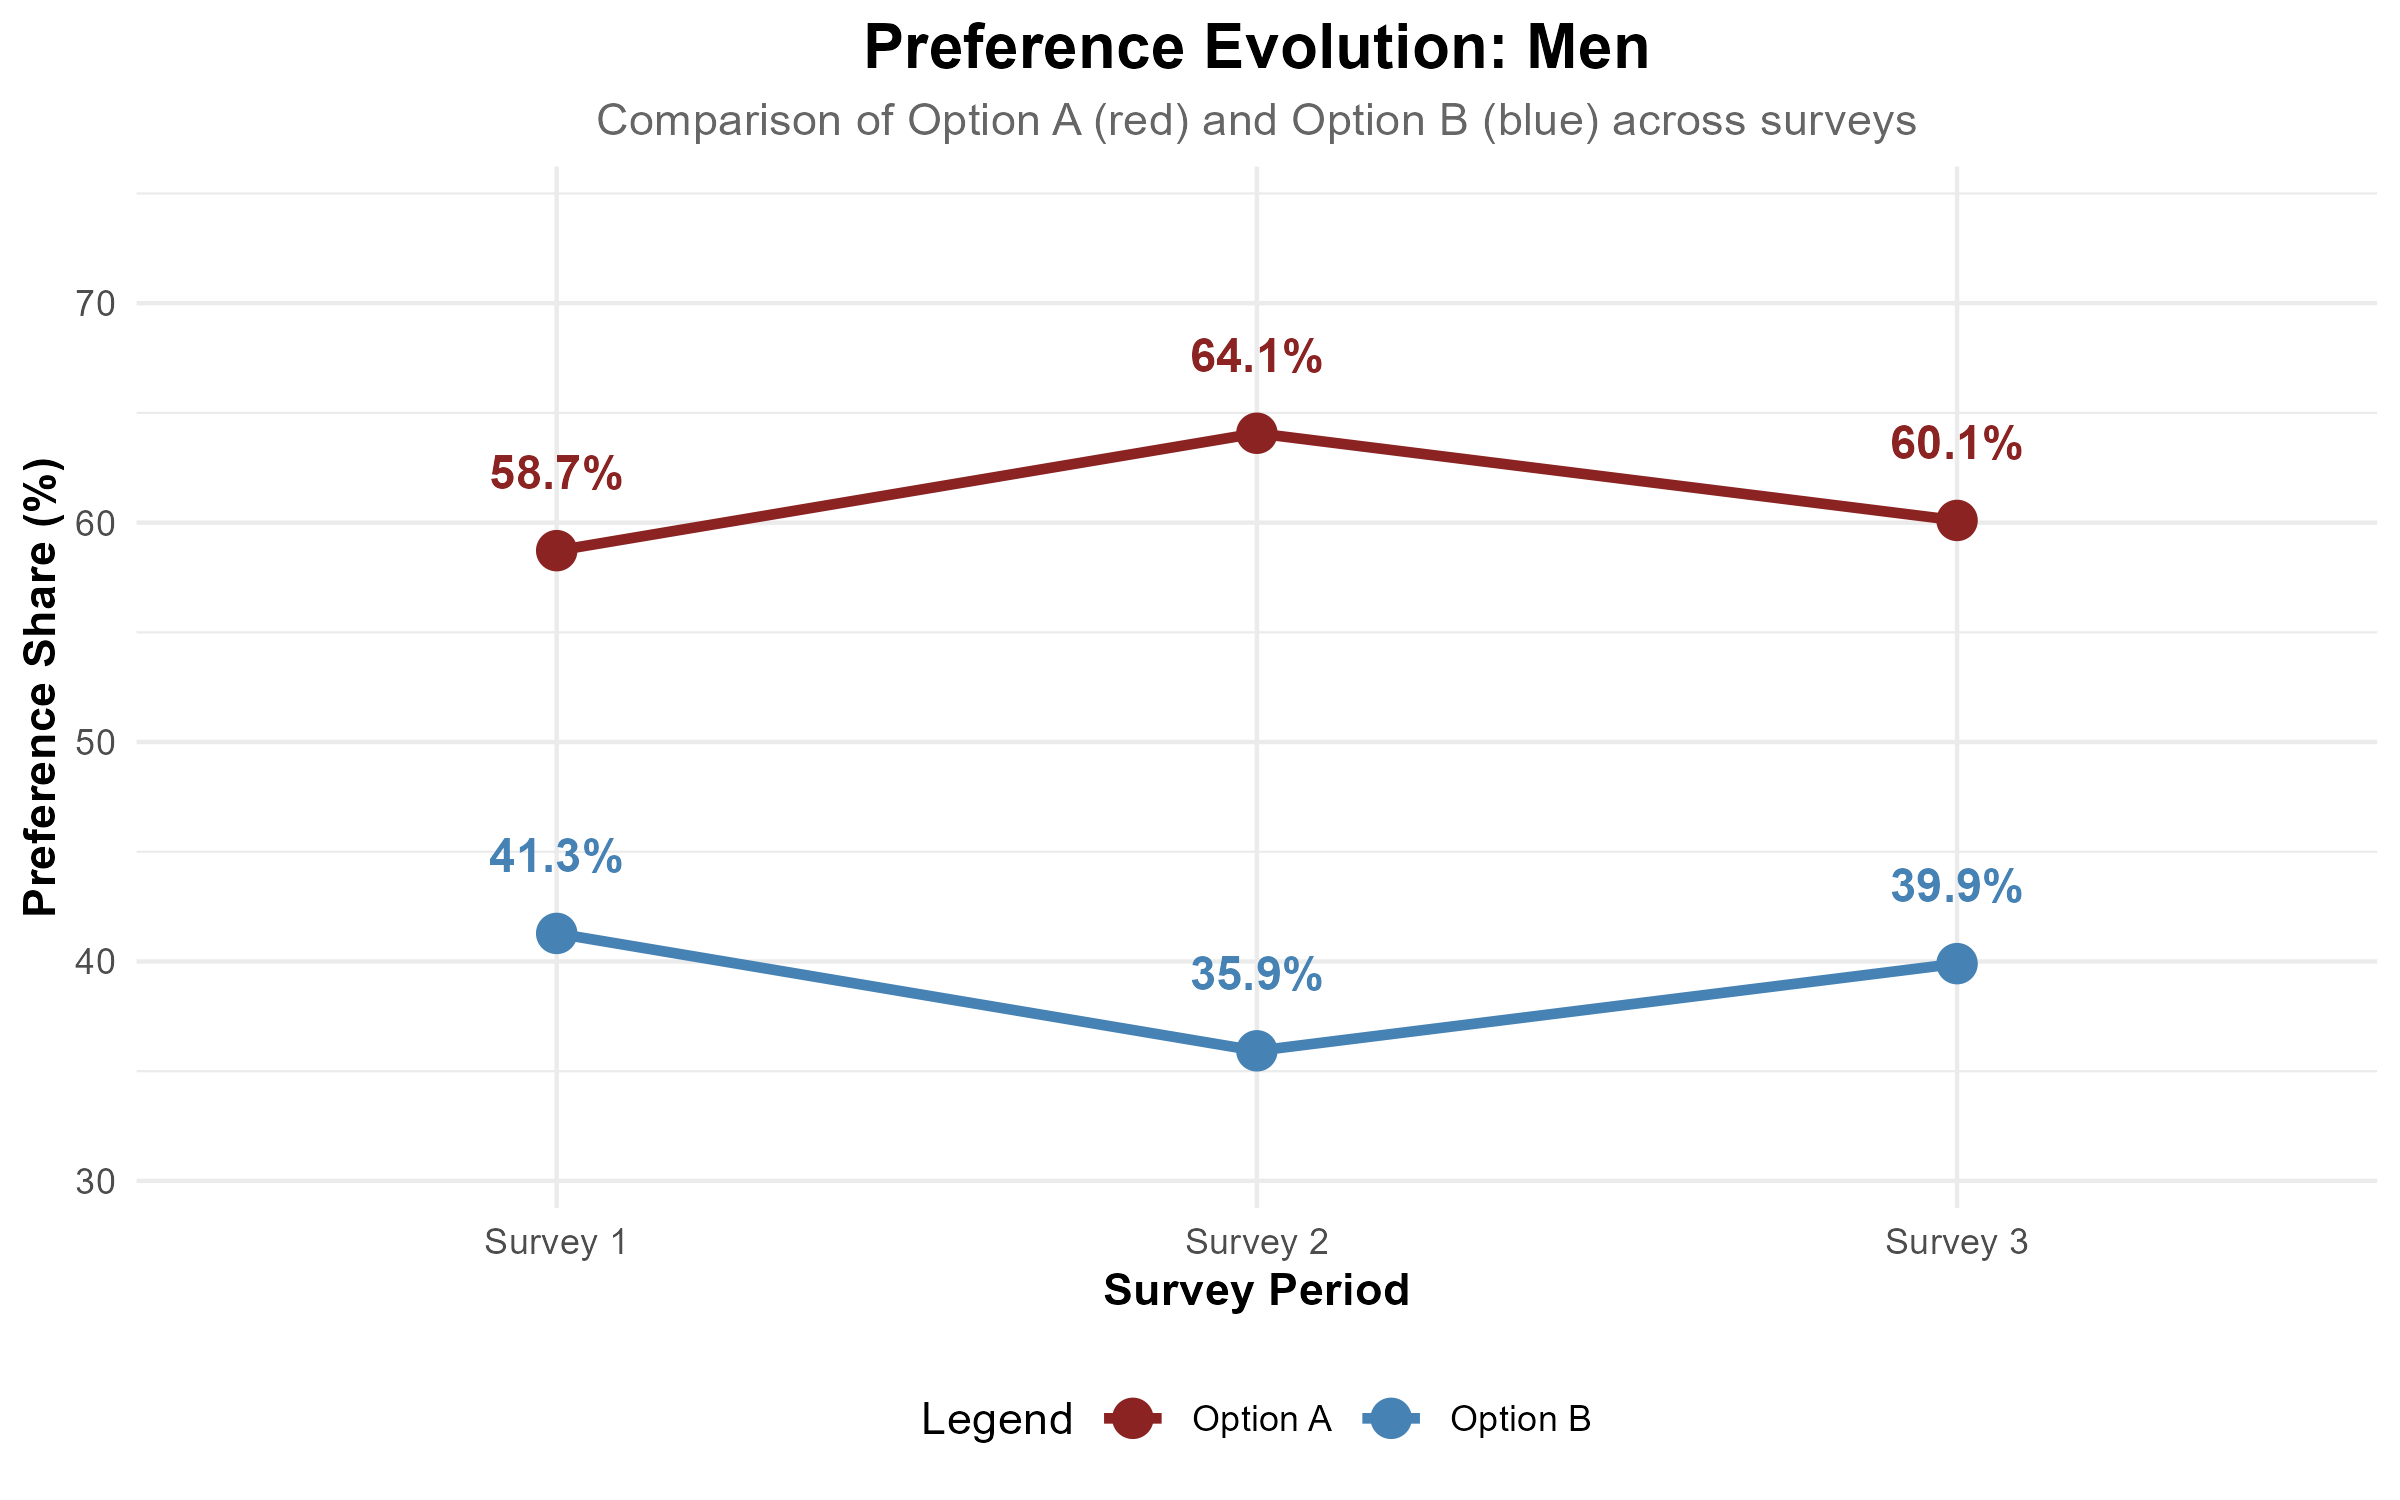
\includegraphics[width=0.8\linewidth]{figs/evolution_preference_share_men}
	\end{figure}
\end{frame}

\begin{frame}{Evolution of preference share for women}
	\begin{figure}[h!]
		\centering
		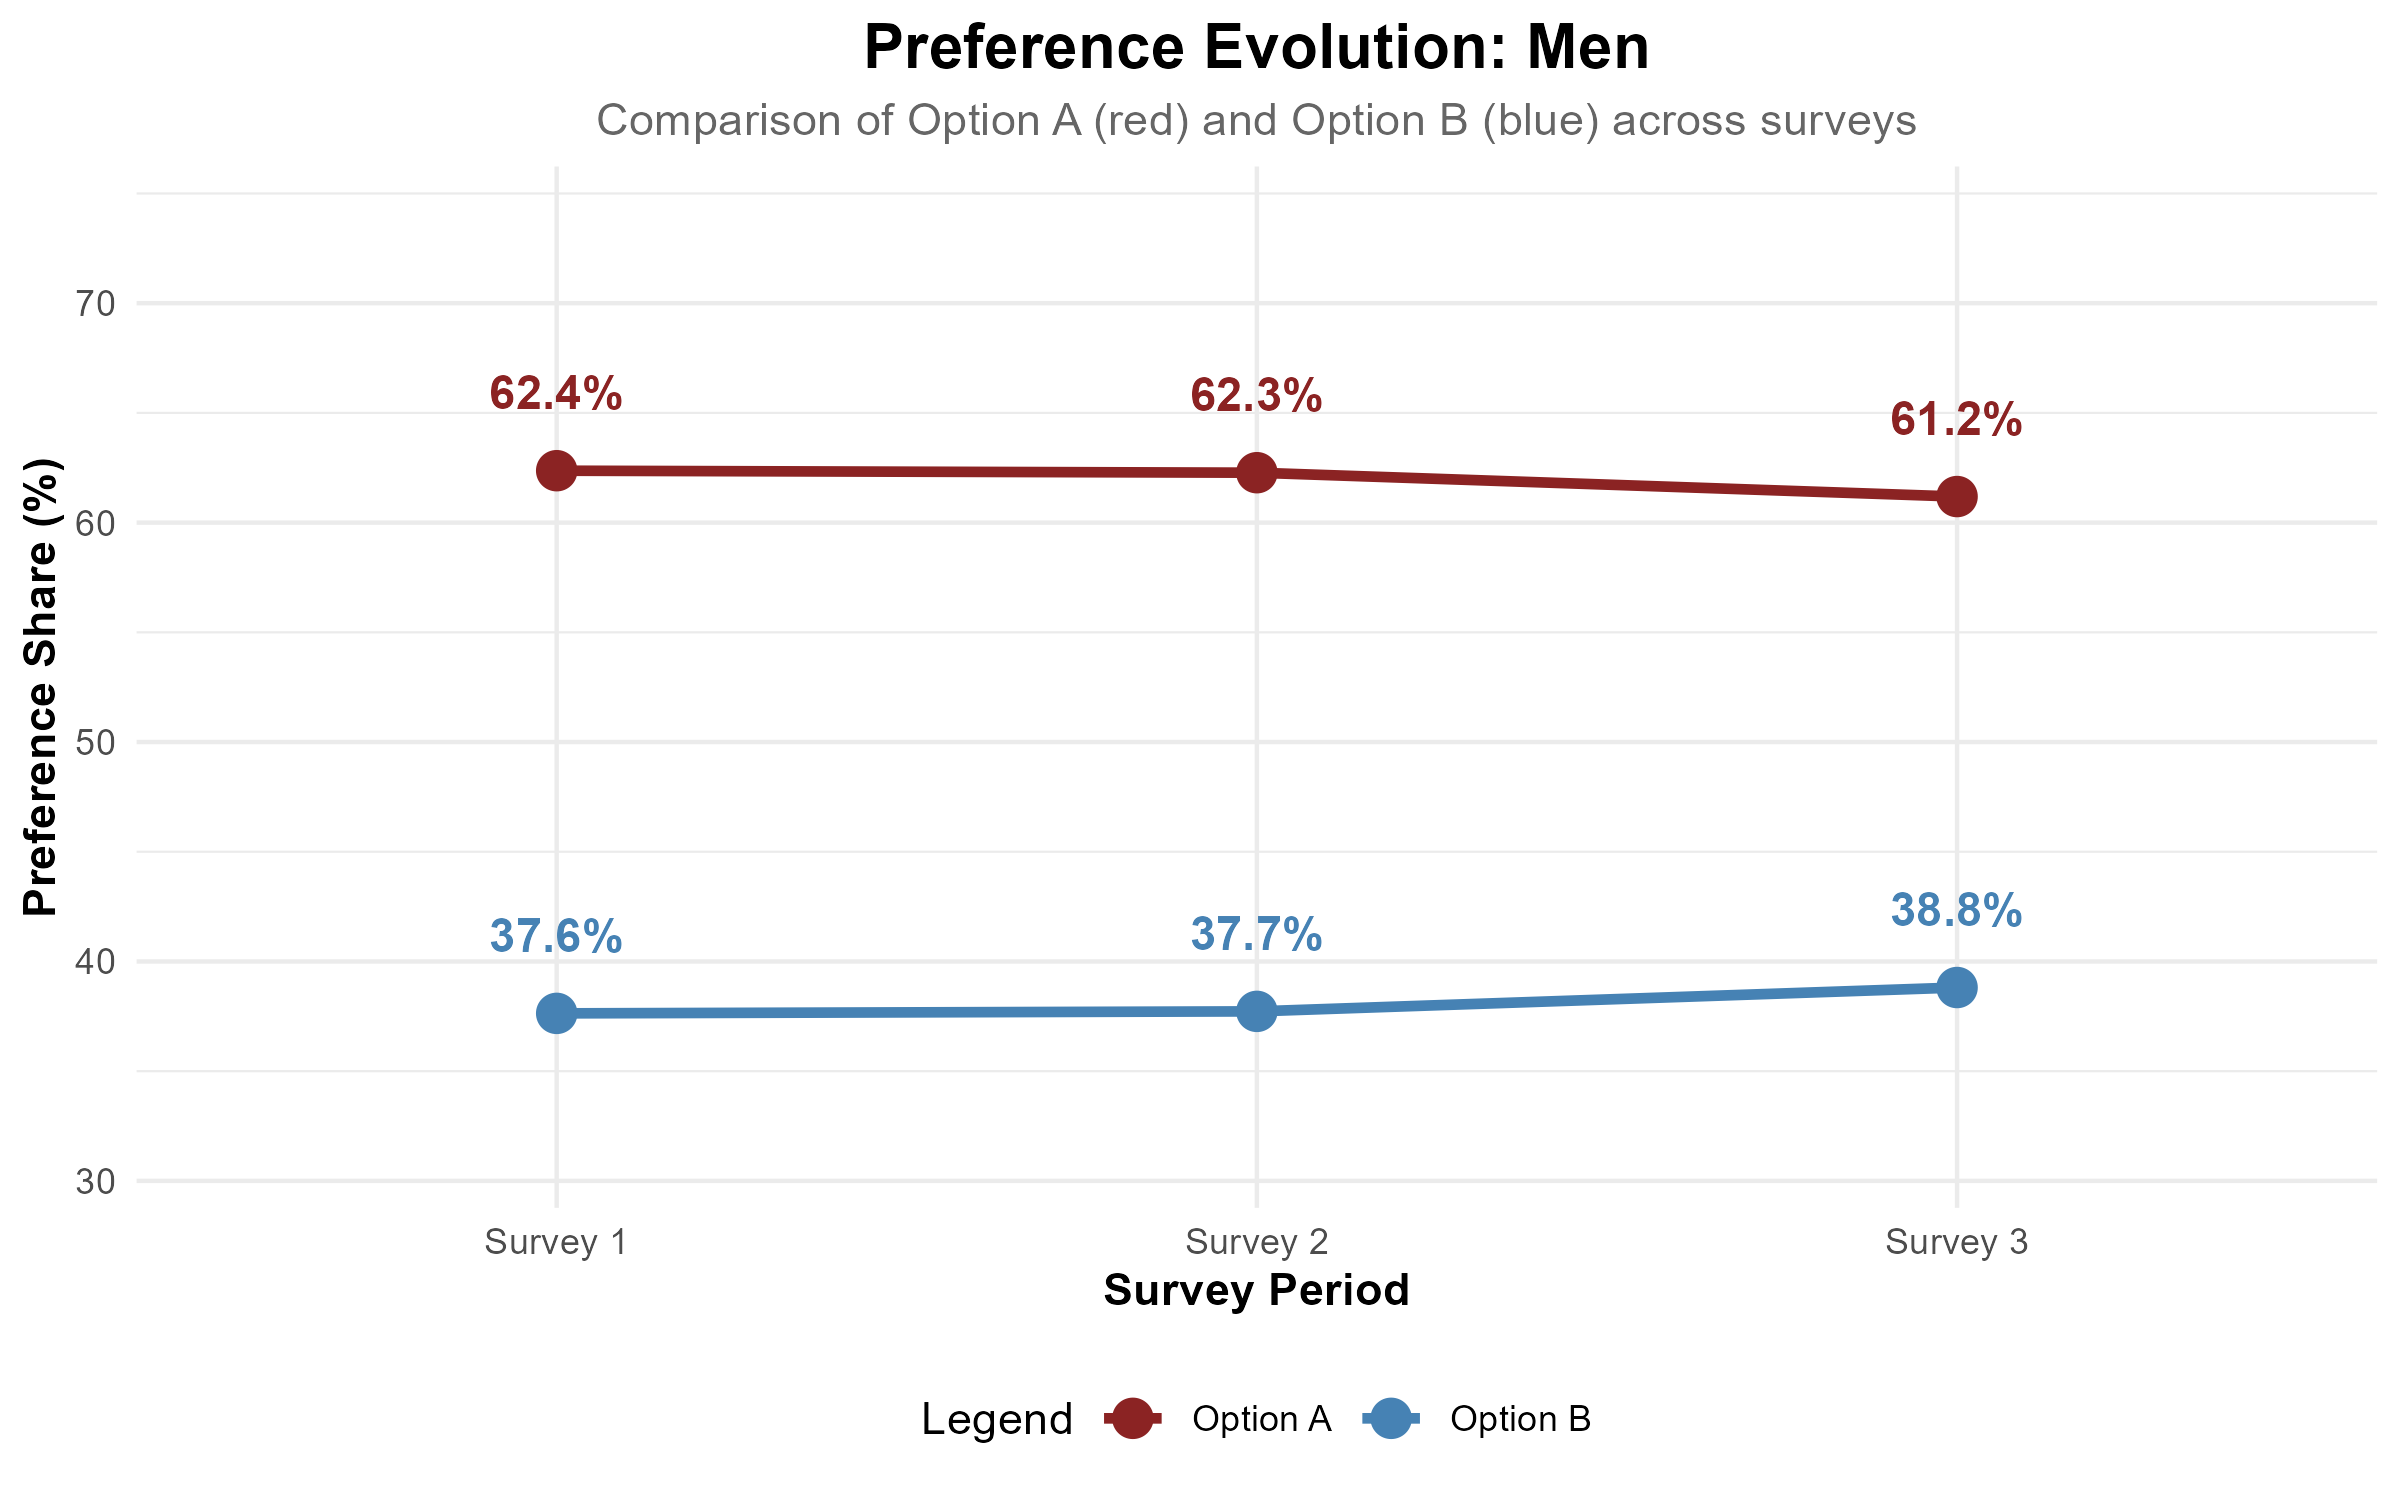
\includegraphics[width=0.8\linewidth]{figs/evolution_preference_share_women}
	\end{figure}
\end{frame}

\begin{frame}{Age groups in electorate}
	The population is divided in four age groups, starting at 17 years old. The age share for the electorate on a nationwide level is shown in the following table, which is replicated in the polls by the use of a weighting factor. This proportion is maintained for the three surveys. 
	\begin{table}
		\resizebox{0.4 \textwidth}{!}{
		\begin{tabular}{c c}
			\toprule
			\textbf{Age group} & \textbf{\% of electorate} \\
			\midrule
			17-24 years old & 16 \\
			\midrule
			25-39 years old & 32 \\
			\midrule
			40-54 years old & 27 \\
			\midrule
			55+ years old & 25 \\
			\bottomrule
		\end{tabular}
	}
	\end{table}
\end{frame}

\begin{frame}[allowframebreaks]{Preference share evolution by age group}
	The data was divided in the four considered age groups and afterwards the preference share for each subgroup was calculated for the three surveys. As such, we can see the change in support for option A and B over the three surveys.
	\begin{table}[h]
		\centering
		\resizebox{0.8 \textwidth}{!}{
		\begin{tabular}{llccc}
			\toprule
			\textbf{Age group} & \textbf{Option} & \textbf{Survey 1 (\%)} & \textbf{Survey 2 (\%)} & \textbf{Survey 3 (\%)} \\ 
			\midrule
			17-24
			& Option A & $59.8$ & $64.2$ & $56.1$ \\
			\midrule
			25-39
			& Option A & $68.2$ & $67.8$ & $65.1$ \\
			\midrule
			40-54 
			& Option A & $61.9$ & $67.6$ & $59.9$ \\
			\midrule
			55+ 
			& Option A & $ 50.8$ & $ 52.4$ & $58.8$ \\
			\bottomrule
		\end{tabular}
	}
	\caption{Preference share evolution for option A by age group.}
	\end{table}
	
	\begin{table}[h]
		\centering
		\resizebox{0.8 \textwidth}{!}{
			\begin{tabular}{llccc}
				\toprule
				\textbf{Age group} & \textbf{Option} & \textbf{Survey 1 (\%)} & \textbf{Survey 2 (\%)} & \textbf{Survey 3 (\%)} \\ 
				\midrule
				17-24
				& Option B & $40.2$ & $35.8$ & $43.9$ \\
				\midrule
				25-39
				& Option B & $31.8$ & $32.2$ & $34.9$ \\
				\midrule
				40-54 
				& Option B & $38.1$ & $32.4$ & $40.1$ \\
				\midrule
				55+ 
				& Option B & $49.2$ & $47.6$ & $41.2$ \\
				\bottomrule
			\end{tabular}
		}
		\caption{Preference share evolution for option B by age group.}
	\end{table}
\end{frame}

\begin{frame}{Evolution of preference share for A by age group}
	\begin{figure}[h!]
		\centering
		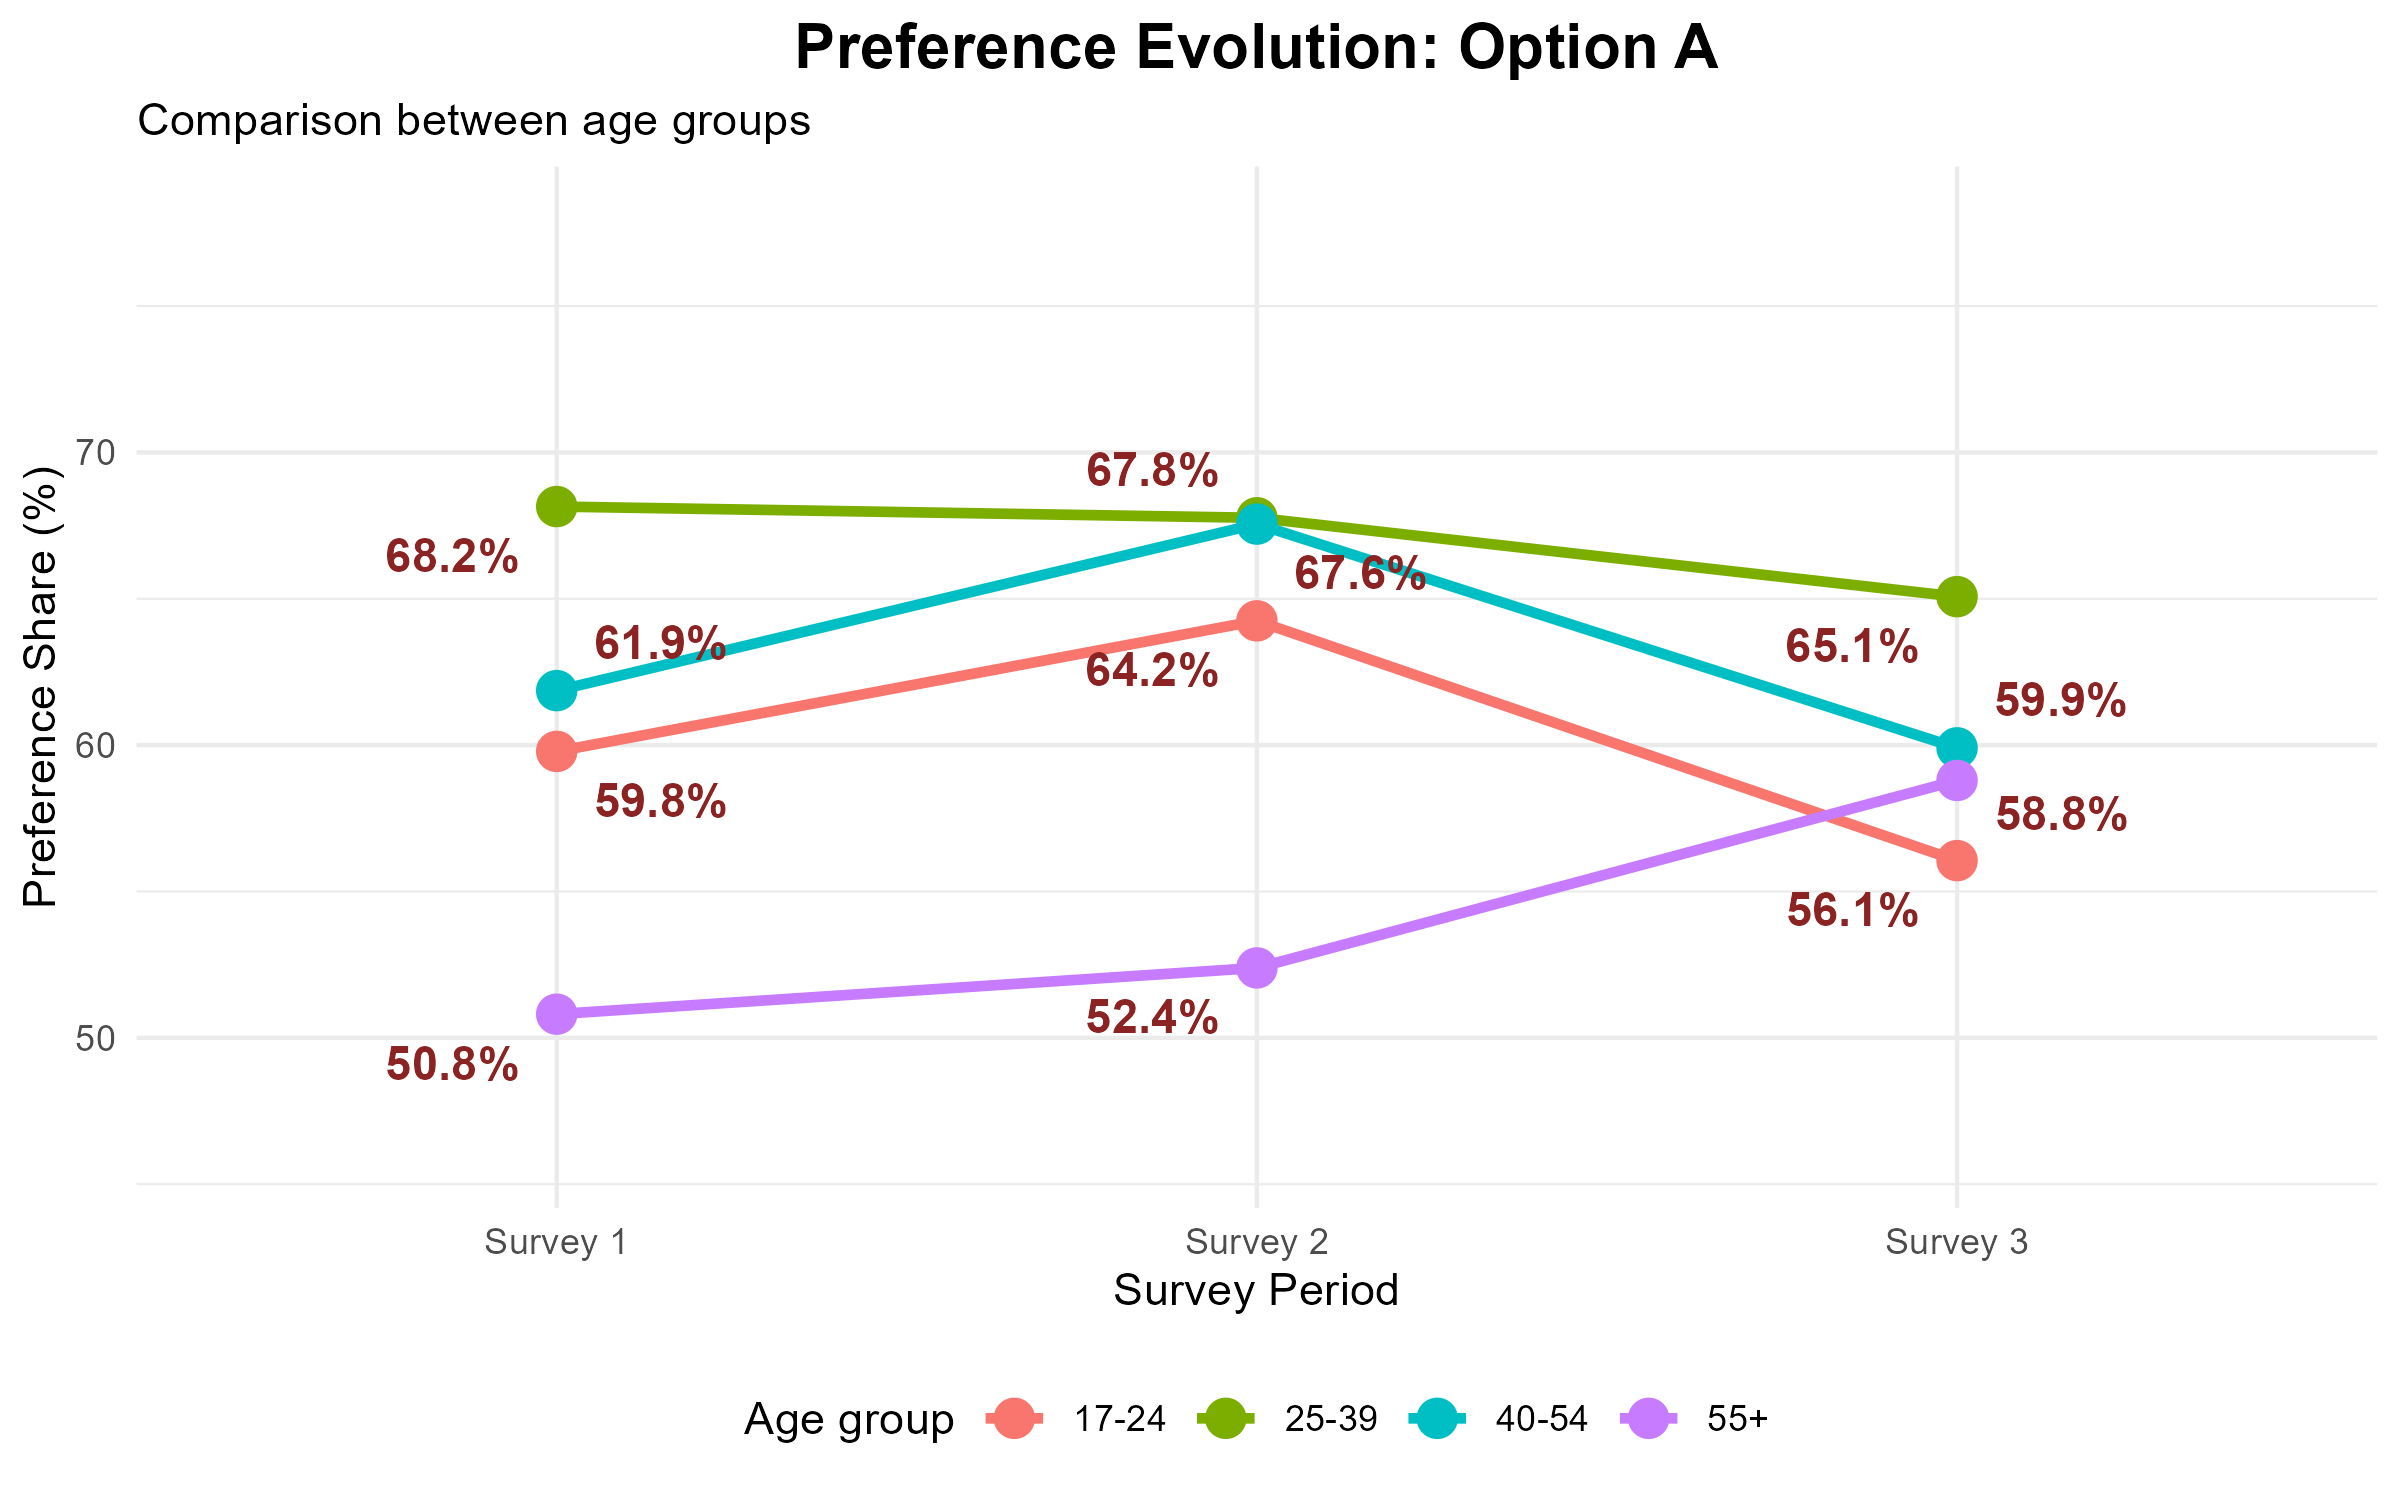
\includegraphics[width=1\linewidth]{figs/evolution_preference_share_A_age}
	\end{figure}
\end{frame}

\begin{frame}{Evolution of preference share for B by age group}
	\begin{figure}[h!]
		\centering
		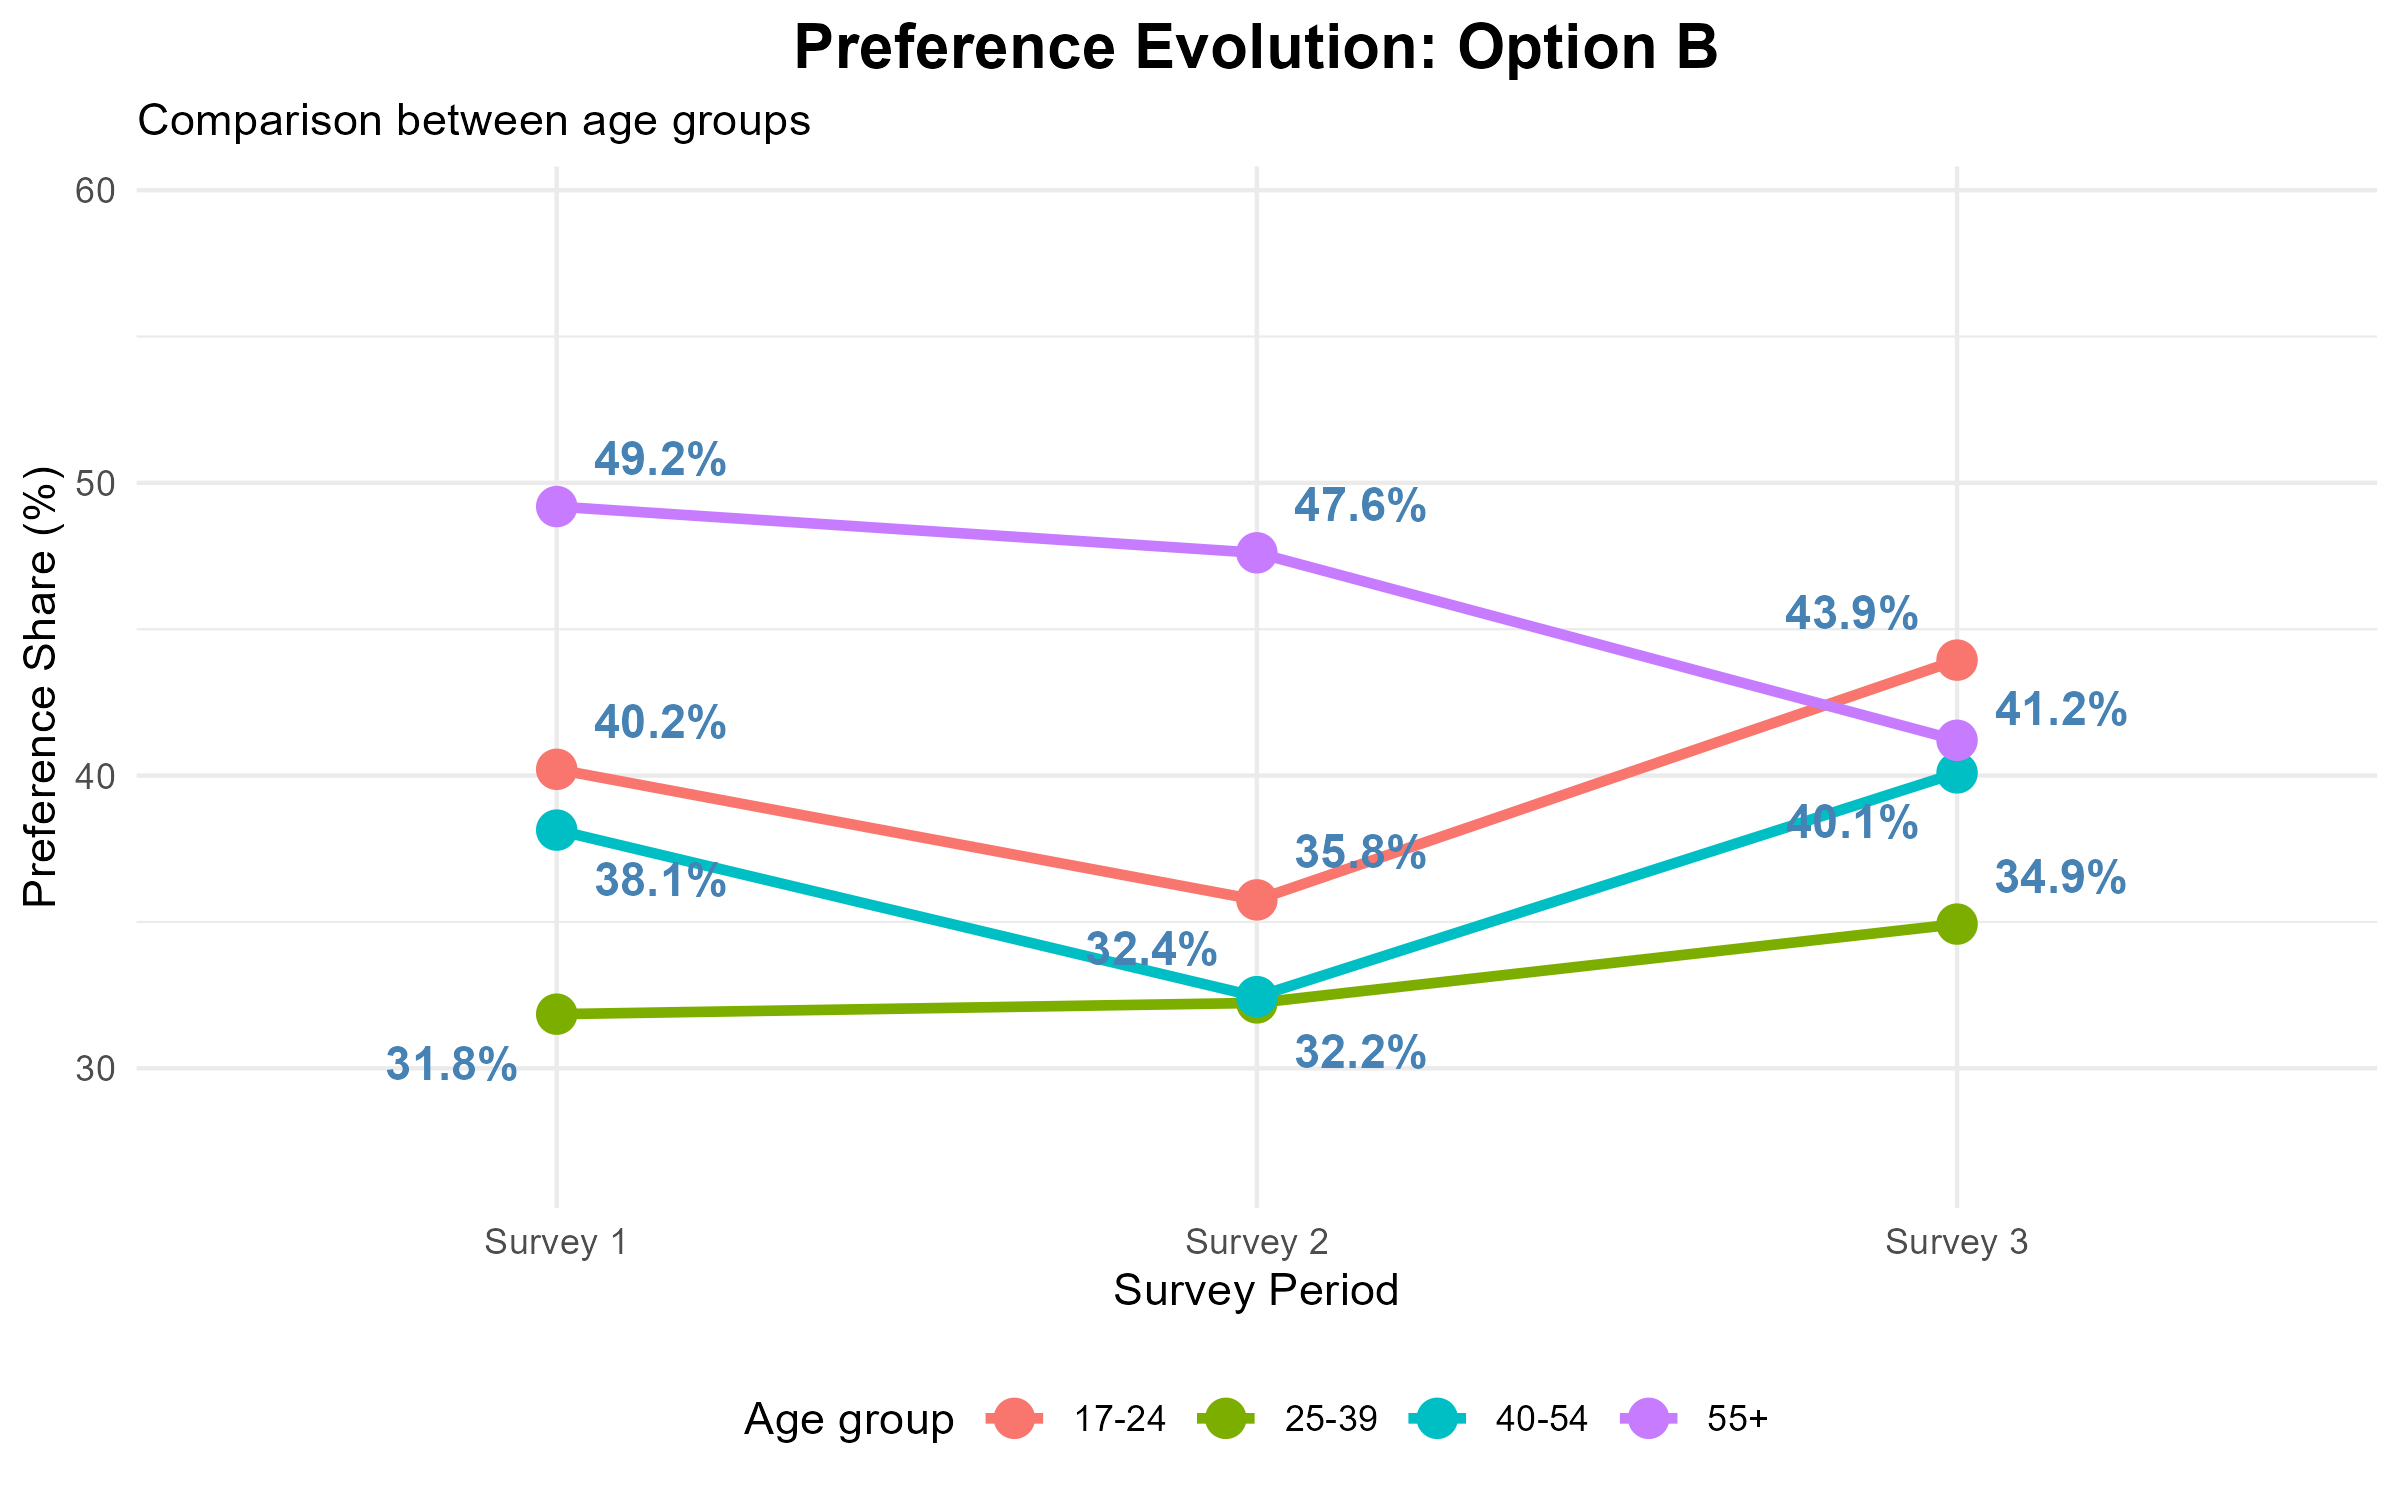
\includegraphics[width=1\linewidth]{figs/evolution_preference_share_B_age}
	\end{figure}
\end{frame}


%TODO:
% - Hacer el analisis de los datos por tipo de influencia, viendo el patron por edad
% - Graficar, notando que solo reflejan el cambio de opinion global
% - Grafica de la diferencia de preferencia por genero, viendo que se mantiene casi constante todo el periodo evaluado
% - Lo mismo para un modelo unicamente con edades
\section{Bibliography}
\begin{frame}[allowframebreaks]{Bibliography}
	\bibliographystyle{plain}
	\bibliography{fuentes}
\end{frame}
\end{document}}